\section{Zadání}

Uvažujte přímkový model s nenormální náhodnou residuální složkou.
Pomocí simulační studie porovnejte vlastnosti odhadů parametrů modelu získaných metodou nejmenších čtverců, metodou ortogonální regrese, metodou LAD a metodou jádrové regrese.

\subsection{Alternativní zadání}

Pro reálná data odhadněte parametry modelu metodou nejmenších čtverců, metodou ortogonální regrese, metodou LAD a metodou jádrové regrese a výsledné odhady porovnejte.

\section{Data}

Pro vypracování semestrální práce jsme zvolili první variantu dat.
Zadefinovali jsme tedy lineární model s koeficienty \( \beta_0 = 2 \), \( \beta_1 = 1 \) a přičetli k němu náhodnou veličinu vygenerovanou z \( X^2 \) rozdělení o dvou stupních volnosti.

\begin{figure}[htb]
    \centering
    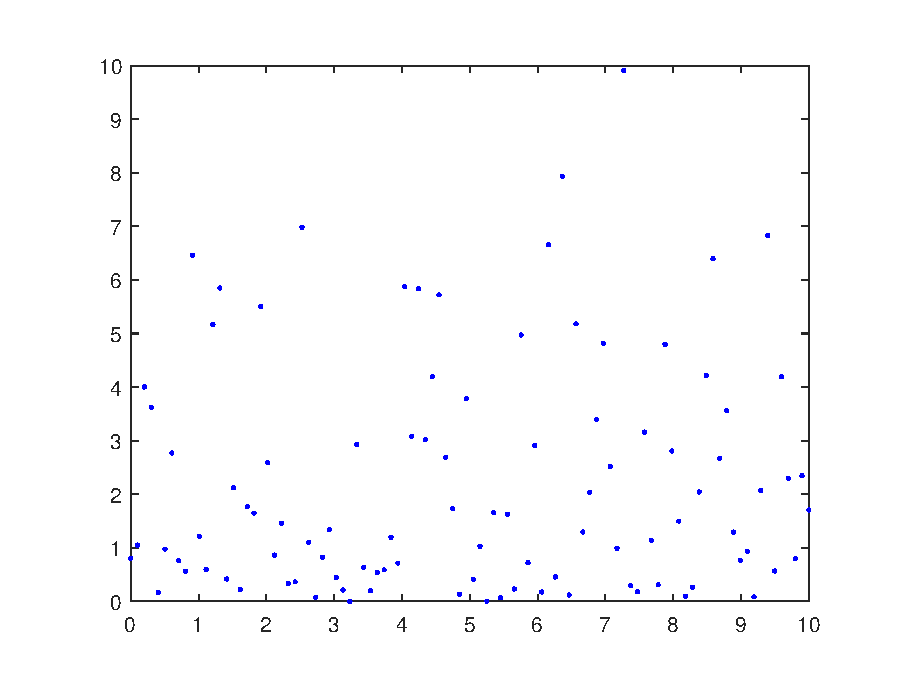
\includegraphics[width=0.7\textwidth]{graphs/fig3.eps}
    \caption{Náhodná veličina vygenerovaná z \( X^2 \) rozdělení}
    \label{fig:lr3}
\end{figure}
\FloatBarrier

\section{Vypracování}

Odhladli jsme parametry modelu, dle zadání, metodami:

\begin{itemize}
    \item nejmenších čtverců,
    \item ortogonální regresí,
    \item LAD.
\end{itemize}

Výsledky jsou k videní na grafu~\ref{fig:lr1}.

\begin{figure}[htb]
    \centering
    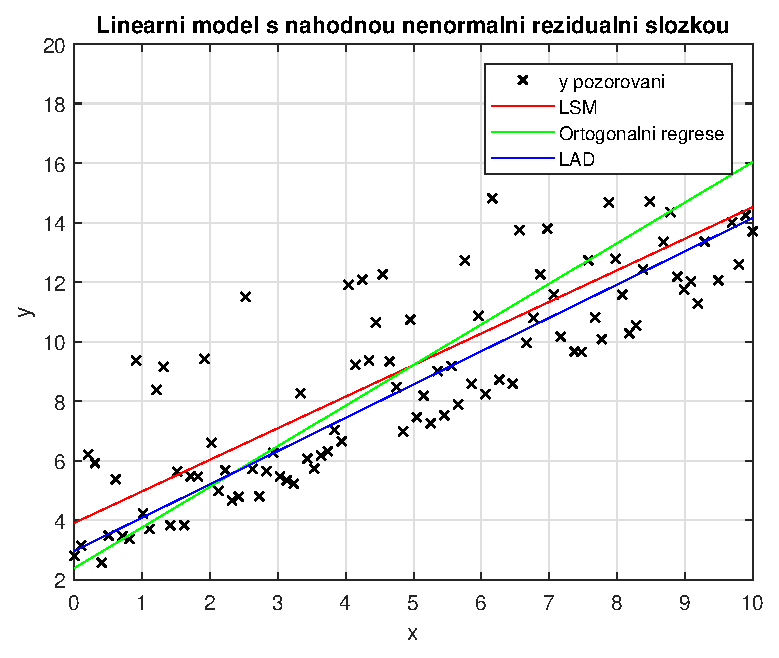
\includegraphics[width=0.7\textwidth]{graphs/fig1.eps}
    \caption{Výsledné křivky po parametrických odhadech každou ze zadaných metod}
    \label{fig:lr1}
\end{figure}
\FloatBarrier

Na první pohled není zřetelné, která metoda odhadla parametry modelu nejlépe.
Pro takové výsledky bychom museli provést test.
Například test kumulativní Eukleidovské vzdálenosti všech simulovaných bodů od generovaných přímek.

Kdybychom však chtěli vědět, která metoda nejlépe odhadla parametry původní, nezašuměné přímky, můžeme se podívat na odhadnuté parametry.

\begin{equation*}
    \left[ \begin{matrix} \beta_{LSE} \\ \beta_{Orto} \\ \beta_{LAD} \end{matrix} \right] = \left[ \begin{matrix} 3.9159 & 1.0600 \\ 2.4010 & 1.3630 \\ 2.9753 & 1.1175 \end{matrix} \right]
\end{equation*}

Se znalostí původního parametru \( \beta \) se jednoduše dopočteme Eukleidovské normy od původního vektoru.

\begin{align*}
    \left\lVert \beta - \beta_{LSE} \right\rVert &= 1.9168 \\
    \left\lVert \beta - \beta_{Orto} \right\rVert &= 0.5409 \\
    \left\lVert \beta - \beta_{LAD} \right\rVert &= 0.9824
\end{align*}

V druhé části práce jsme data odhadovali neparametrickou metodou jádrové regrese.
Z grafu vidíme, že křivka data popisuje lépe než předešlé metody, nedostáváme však konkrétní parametr \( \beta \).

\begin{figure}[htb]
    \centering
    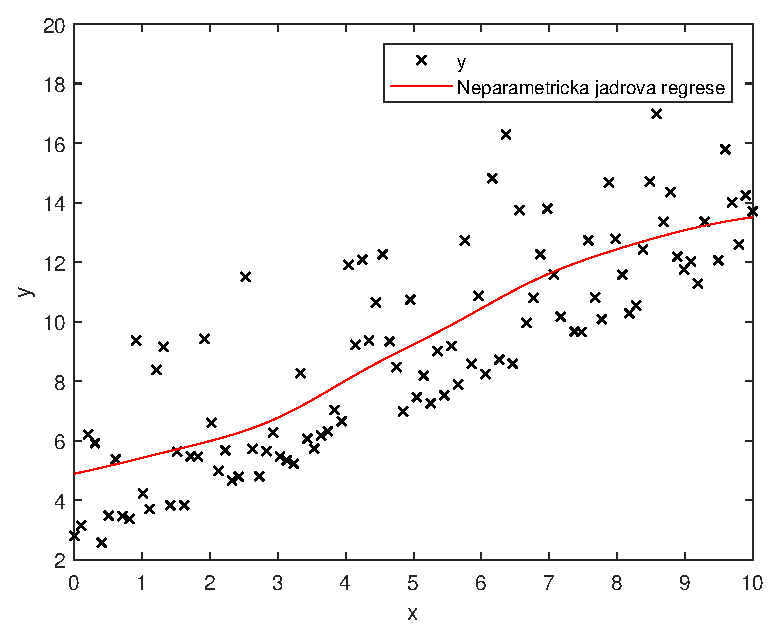
\includegraphics[width=0.55\textwidth]{graphs/fig2.eps}
    \caption{Neparametrická jádrová regrese}
    \label{fig:lr2}
\end{figure}
\FloatBarrier

\section{Závěr}

V semestrální práci jsme se podívali na vlastnosti několika metod pro odhad parametrů modelu.
Dle výsledů první části příkladu bychom mohli udělat závěr, že dle metriky Eukleidovské normy nejlépe parametry původní křivky odhadne metoda Ortogonální regrese.

V druhé části práce jsme získali křivku, které dobře interpoluje zadaná data.
Při znalosti původní (lineární) funkce však můžeme říci, že tato data hůře extrapoluje.
Krom toho tato metoda je neparametrická, potenciálně získatelné koeficienty \( \beta \) jsou tedy funkčně závislé.
